%! Author = mariuszindel
%! Date = 25.01.21

\section{Verschlüsselung}




\section{RSA}
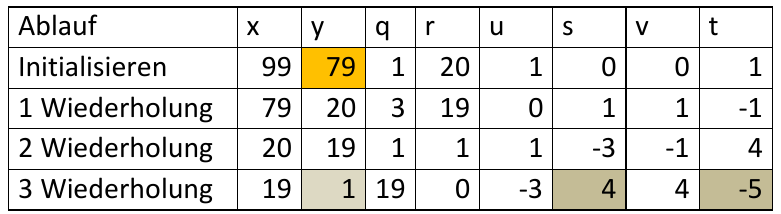
\includegraphics[width=\linewidth]{graphic/extern-reto/RSA.png}
\begin{itemize}
    \item 99 = $\phi(n)$
    \item 79 = privater Schlüssel
    \item 3. Wiederholung \colorbox{gray}{-5}: Inverse, Somit 99 - 5 = 94
    \item 3. Wiederholung \colorbox{lightlightgrey}{1}: ggT
    \item $s = u_{-1} - q_{-1} * s_{-1}$
    \item $t = v_{-1} - q_{-1} * t_{-1}$
    \item Verschlüsselung: $c = m^{Inverse} $ mod $ n$
    \item Entschlüsselung: $m = c^{79}$mod $n$
\end{itemize}
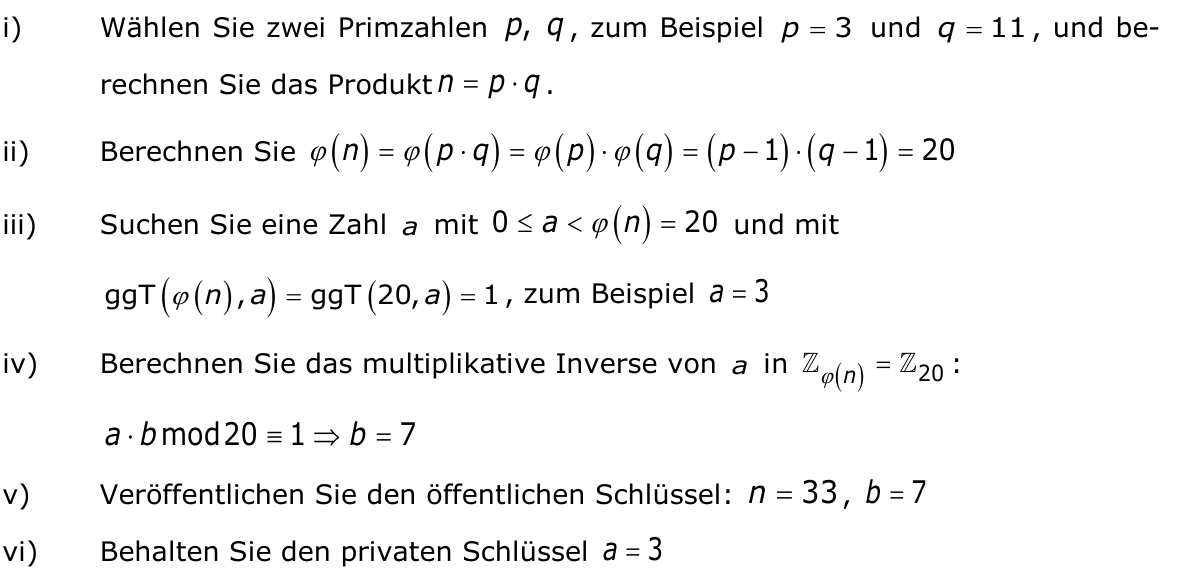
\includegraphics[width=\linewidth]{graphic/extern-reto/RSASchritte.png}



